\newcommand{\nbsp}{\vspace{5mm}}
\newcommand{\suchthat}{\mid}
\newcommand{\eqc}{\overline}	% TODO insert ()'s automagically?
%\newcommand{\eqc}[1]{\overline(#1)}
\newcommand{\inv}[1]{#1^{-1}}
\newcommand{\fxnto}{\rightarrow}
\newcommand{\pp}{\varphi}	% random phi symbol
\newcommand{\pstar}{\pp^*}	% p upper star
\newcommand{\of}{\circ}		% fxn composition
\newcommand{\zero}{\mathbb{0}}
\newcommand{\one}{\mathbb{1}}
\newcommand{\intersect}{\cap}
\newcommand{\union}{\cup}

\newcommand{\N}{\mathbb{N}}
\newcommand{\Nplus}{\N^{> 0}}

\newcommand{\Z}{\mathbb{Z}}
\newcommand{\Zplus}{\Z^{\ge 0}}
%\newcommand{\ZZ}{\Z \times \Z}
\newcommand{\ZZ}{\Z^2}

\newcommand{\Q}{\mathbb{Q}}

\newcommand{\R}{\mathbb{R}}
%\newcommand{\RR}{\R \times \R}
\newcommand{\RR}{\R^2}

\newcommand{\Zpx}{\Z_p^\times}

\newcommand{\vectI}[1]{(#1_1, ..., #1_n)}
\newcommand{\vectII}[2]{(#1_1 + #2_1, ..., #1_n + #2_n)}
\newcommand{\vectIII}[3]{(#1_1 + #2_1 + #3_1, ..., #1_n + #2_n + #3_n)}
  
\documentclass[12pt]{article}
\usepackage{amsmath}
\usepackage{amsfonts}
\usepackage{amsthm}
\usepackage{fullpage}
\usepackage[pdftex]{graphicx}
\usepackage{cite}
\usepackage{url}
\usepackage{listings}
 

\newcommand{\HRule}{\rule{\linewidth}{0.5mm}}

\everymath{\displaystyle} \newcommand{\code}[1]{\texttt{#1}}

%\title{Client-Driven Pointer Analysis in LLVM} 
%\author{Dustin "Reaching Def" Carlino \and Kurt "raw\_stream" Scherer \and Parth "Flow
%Insensitive" Upadhyay \and Jason "Def Without a Use" Wolfe}
%\date{}

\begin{document} 

\begin{titlepage}

\begin{center}


% Upper part of the page
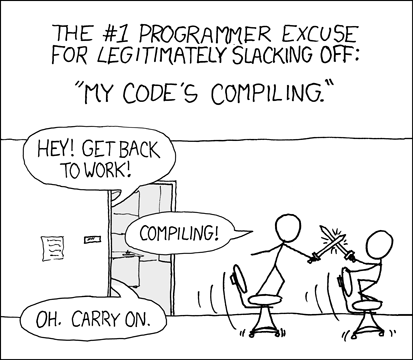
\includegraphics[width=0.60\textwidth]{images/xkcd_comic_2}\\
\textsc{Image Credit: \url{www.xkcd.com}}\\[1cm]    

\textsc{\LARGE University of Texas at Austin}\\[1.0cm]

\textsc{\Large Final Project}\\[0.5cm]


% Title
\HRule \\[0.4cm]
{ \huge \bfseries Client-Driven Pointer Analysis in LLVM }\\

\HRule \\[1.5cm]

% Author and supervisor
\begin{minipage}{0.5\textwidth}
\begin{flushleft} \normalsize
\emph{Author:}\\
Dustin \textsc{``Reaching Def"} Carlino\\
Kurt \textsc{``raw\_stream"} Scherer\\
Parth \textsc{``Flow Insensitive"} Upadhyay\\
Jason \textsc{``Def Without a Use"} Wolfe
\end{flushleft}
\end{minipage}
\begin{minipage}{0.4\textwidth}
\begin{flushright} \large
\emph{Advisor:} \\
Dr.~Calvin \textsc{Lin}
\end{flushright}
\end{minipage}

\vfill

% Bottom of the page
{\large \today}

\end{center}

\end{titlepage}


\tableofcontents
\listoffigures
\newpage

%%%%%%%%%%%%%%%%%%%%%%%%%%%%%%%%%%%%%%%%%%%%%%%%%%%%%%%%%%%%%%%%%%%%%%%%%%%%%%%%

\section{Introduction}

In his $2003$ thesis, Samuel Guyer presented the {\bf Broadway Compiler}, a
compiler that could take advantage of the {\em semantics} of library calls to
perform optimizations \cite{guyer}. This compiler was built on the premise that
libraries are domain specific languages, and that many existing optimization
algorithms could work equally well for library calls. The compiler is typically
unable to perform these optimizations without more information about what these
library calls are actually doing.

To perform such analyses, Guyer shows that a powerful pointer analysis framework
is needed, and he introduces a novel method of client-driven pointer analysis
where the specific needs of the client drive the needs of the pointer
analysis.

While the ideas behind this project are still valid today, the project has gone
largely unmaintained. The goal behind our project is to apply the ideas from
Broadway in a modern compiler: LLVM.

We assume familiarity with the general concepts of pointer analysis, context-
and flow-sensitivity, and iterative data-flow analysis (IDFA).

%%%%%%%%%%%%%%%%%%%%%%%%%%%%%%%%%%%%%%%%%%%%%%%%%%%%%%%%%%%%%%%%%%%%%%%%%%%%%%%%

\section{Project Scope and Approach}

The specific portion of this task we undertook was porting the client-driven
pointer analysis. The original scope of our project included:

\begin{itemize}
\item A fast but imprecise flow/context-insensitve pass 1 
\item A monitor to record loss of precision 
\item An adapter to use the information from the monitor 
\item A general IDFA
\end{itemize}

The scope proved to be too ambitious, however, and we were unable to complete
all of the goals we set out to. We were able to complete the general IDFA and
the flow/context-insensitive pass as an extension upon the general IDFA with
toggle-able sensitivity in either dimension.

Our approach to porting made use of the availability of the original source code.
``Clean room reverse-engineering'' just by using information from papers may have
led us to a cleaner design, but it is unlikely we would have implemented as much
of our feature set. There are some significant design details omitted from
published papers that are documented in the source. A goal of this report is to
make those more clear.

%%%%%%%%%%%%%%%%%%%%%%%%%%%%%%%%%%%%%%%%%%%%%%%%%%%%%%%%%%%%%%%%%%%%%%%%%%%%%%%%

\section{Program Model}

Our program model closely mimics that which was presented in the thesis. However
we will explain our understanding and also outline where we deviate from the
thesis.

The thesis \cite{guyer} describes most algorithms in appropriate detail. Section
3.7 describes the changes needed for LLVM. The goal of this section is to
discuss the main objects/structures used.  We will not repeat explanations of
the general algorithms.

We will first give an overview that briefly explains and motivates each
structure. Then we will give details on each.

\subsection{Big Picture}

Our aim is for this section to exclusively enable understanding of the
algorithms presented in Guyer's thesis, as well as some of those establish by
the corresponding code and not necessarily explicitly discussed in the thesis.

The goal is to construct a framework capable of performing context-sensitive
(C.S.) and flow-sensitive (F.S.) dataflow analysis. Flow-insensitive (F.I.) and
context-insensitive (C.I.) analysis will be degenerate cases of the general
engine. Let Memory Blocks (``memblocks'', ``blocks'', ``MBs'') represent stored
memory, whether it's ``normal'' integer variables on the stack or heap memory.
The flow values we will operate on are points-to sets of a MB, meaning one MB
can point to a set of MBs.

Traditional iterative data-flow analysis computes and stores flow values at
every program point. This is actually quite redundant; it suffices to store the
flow value only when it changes. To encode flow-sensitivity, we create a
Definition (``def'') whenever a MB's flow value changes. At any program point, we
can find the reaching def that gives the answer at that point.

What is meant by ``program point''? Procedures contain basic blocks, and basic
blocks contain statements: so one answer is any of these levels of granularity.
However, we also wish to encode context-sensitivity. We want to remember the
full call graph from the main() root, rather than the single-level static
call-site or any kind of k-limiting. So we can form a tree of Locations:
Procedure Locations (``Proc Loc'') have Basic Block Locations (``BB Loc'') as
children, and BB Locs have Statement Locations (``Stmt Loc'') as children. The
recursive step that gives us C.S. is the optional child of a Stmt Loc: at a
procedure call, the Stmt Loc will have a Proc Loc as a child. If the same
procedure is called multiple times, it will always have a different Stmt Loc for
a parent. This parent is not just the static call-site, but the
dynamic call-site. This formulation of Locations is equivalent to cloning
procedures.

So we have Memory Blocks with Defs established at Locations. At any Location, we
can find the reaching def and get the correct flow value. All MBs are managed by
a ``Memory Table'' that indexes MBs by LLVM SSA value and Proc Loc. When we call a
procedure from one location, a local variable may have Defs at various
Locations. When we call the procedure from another place, that same local
variable should have a different set of Defs. Thus, the Memory Table does need
both LLVM value and Proc Loc.

\subsection{Locations}

To encode context-sensitivity, we use the method prescribed in the thesis which
involves a tree structure consisting of 3+1 types of nodes:

\begin{itemize}
\item Statement Locations (\code{Stmt\_Loc}) - encode single statements. The
      child is either nothing or a \code{Proc\_Loc}, meaning the \code{Stmt\_Loc} is a
      call-site.
\item Basic Block Locations (\code{BB\_Loc}) - encode basic blocks. The children
      of a \code{BB\_Loc} are \code{Stmt\_Loc}s that represent the statements
      contained within the basic block.
\item Procedure Locations (\code{Proc\_Loc}) - encode procedures. The children
      of a \code{Proc\_Loc} are \code{BB\_Loc}s that represent the basic blocks
      contained with the procedure.
\item Global Locations (\code{Global\_Loc}) - encode globals. These aren't really in
      the tree (no children, no parents), but are used in the same fashion as the 
      rest of the \code{Loc} instances.
\end{itemize}

To encode {\bf context sensitivity}, one simply creates a new \code{Proc\_Loc}
for every function call. The parent of the Proc Loc encoding the root main()
function is null. (It is assumed that no program ever invokes main recursively.)
To encode {\bf context insensitivity}, refer to the same \code{Proc\_Loc} for
every call to a procedure.

\subsubsection{Dominance Testing}

Finding reaching defs involves making many queries about whether one Location
dominates another. Guyer describes an intuitive constant-time numbering scheme
for testing the dominates relation. It is difficult to assign the numberings
because more Locations are instantiated as procedure calls are analyzed. He
mentions an online formulation of this algorithm, but does not detail it.
Nothing resembling it appears in the C-Breeze source.

We instead modified the approach used in C-Breeze. Within the same static procedure,
answering dominance queries about two statements or basic blocks is trivial --
there is even an LLVM pass that does it. Given two Locations of depth $m$ and
$n$, we can find their common parent in $O(max(m, n))$ by chasing the deeper
Location's parent pointer until the depths are equal, and then chasing both
parent pointers simultaneously. The common parent is either a basic block
(meaning we have the two Locations as Stmt Locs) or a procedure (meaning we have
two BB Locs). At this point, the static LLVM dominator relation can be applied.

In the C.I. case, a Proc Loc's parent will be null. The dominates relation is
never true for Locations inside two different C.I. Proc Locs. Finding reaching
defs in the presence of C.I. calls is slightly more complicated and may not be
implemented correctly.

\subsubsection{Globals}

In LLVM, globals are declared and optionally initialized by a special \code{global} 
instruction in the IR. Because they're constant throughout the program, we simply
iterate through them before analysis creating \code{Global\_Loc}s and \code{Mem\_Def}s
for them. Because globals are visible anywhere, they also necessitate a simple change
to the dominate test, to the effect that they strictly dominate everything except 
other globals.

\subsection{Memory Blocks}

A Memory Block (\code{Mem\_Block}) represents anything that can point or be
pointed to. This manifests as a normal scalar variable on the stack, a
heap-allocated object, a field of a struct, or a return value from a procedure.
Our representation stores a list of defs, uses (each of which has a reaching
def), and, for structs, a mapping from field to the contained Mem Block.

Our array and heap model follows Guyer's formulation, except for multiple
instance analysis of heap variables (described in Limitations). All assignments
to an array or heap MB is forced as a weak update, since it may represent
multiple objects at run-time.

\subsection{Externals and Virtual PHI Functions}

Virtual phi functions are also introduced whenever a variable external to a
function (anything that isn't a purely local variable) is modified inside of a
function. Because we place virtual phi functions for merge-points at the start
of basic blocks (storing them in the \code{BB\_Loc}), we thus need every
function call to result in a unconditional branch to a new basic block.

We take advantage of the modular nature of LLVM by running a simple custom
pre-pass \code{-split-at-call} that takes care of guaranteeing this. By
requiring this pass, we have a compiler-infrastructure enforced guarantee that
function calls cannot arbitrarily occur in the middle of a basic block.

\subsection{Def/Use}

For \code{Mem\_Block}s we encode def/use information. For defs, we use a
\code{Mem\_Def} structure that contains the \code{Location} of the def and the
set of \code{Mem\_Block}s that it points to. For uses, we use a \code{Mem\_Def}
structure that contains the \code{Location} of the use, and the reaching\_def of
the use.

To adapt our analysis for flow-insensitivity, one must restrict each
\code{Mem\_Block} to having only one def which contains the information of all
the defs it would have had in a flow-sensitive solution \cite{guyer}.

\subsection{Procedure DB}

C-Breeze pre-computes various things per procedure that do not change. We also
adapt this design.

\begin{itemize}
\item Guyer references somebody who shows that IDFA converge faster if the
      all predecessors of a basic block are visited first. We use an LLVM pass to
      compute the reverse post-order order of basic blocks for a procedure. We adapt
      their implementation of an always-sorted worklist using bit-sets.
\item Mappings of call-sites
\item Pre-computed dominance frontiers and ancestor lists
\end{itemize}

\subsection{Interaction with LLVM IR}

Our rules for evaluating expressions differ slightly from C-Breeze's due to
differences in IR.

\begin{itemize}
\item When we see an ALLOCA or GLOBAL command, we treat that as an identifier
      and take an address.
\item A LOAD indicates some type of dereference. We do not compute points-to
      sets for temporary SSA variables; rather, we do all of the work when we
      hit a STORE. We follow the LOADed operand until we hit an identifier. This
      tells our dereference mechanism how many times to expand points-to sets.
\item LLVM ''bitcasts`` always lead to malloc in our tests. In other cases, it
      should be treated as a no-op.
\item GEP (get element pointer) instructions indicate array or struct field
      accesses.
\item CALLs invoke the handling for C.S. or C.I. procedure calls.
\item PHI nodes follow the usual semantic of unioning points-to sets. Note that
      these are not the same as the virtual phis that we insert.
\item Constants are no-ops
\item Arguments indicate when we should look up the reaching def on a special
      Mem Block representing a certain parameter.
\end{itemize}

%%%%%%%%%%%%%%%%%%%%%%%%%%%%%%%%%%%%%%%%%%%%%%%%%%%%%%%%%%%%%%%%%%%%%%%%%%%%%%%%

\section{Testing}

Our original testing plan was to slowly replicate more and more of the original
C-Breeze/Broadway results. Since we were unable to ever build it, we instead
chose to construct small C programs that test a particular property of our
analysis. Some of these programs include:

\begin{itemize}
\item passes0: recognizing in LLVM IR basic source operations like taking an address and
      dereferencing on the left- and right-hand side
\item passes1: weak updates caused by a statically unknown conditional
\item passes2: having a side effect in a called procedure, so that an
      interprocedural phi is placed
\item passes6: verifying struct fields stay separate and array fields all merge
\item testglobal: verifying the behavior of globals
\item testci: smearing arguments and return values in C.S. versus C.I. mode
\item passes10: testing differences between F.S. and F.I. mode
\end{itemize}

Each test produces a non-trivial log detailing the analysis, so we used three
different techniques to evaluate the validity of the output.  We used three
techniques to evaluate the results. Each requires manual inspection of the test
source just once, to determine the appropriate behavior.  This is one reason why
we exclusively used small, specific test cases.

With more time, unit tests for many components would have been a wise option.
Queries like finding procedure ancestors, detecting recursion, and evaluating
location dominance relations would be prime candidates.

\subsection{Log Comparison}

At the end of analysis, the memory table dumps all known Memory Blocks (both
regular and synthetic), describing the points-to set and location of each def.
Once we verify one log is correct, we could commit and use version control to
notice any future changes to that test. This was slightly complicated by the
fact that lots of our data structures are unordered sets (resulting in many
diffs where results are just printed in a different order). Adding a
lexicographic sort on the symbolic names of Memory Blocks alleviates this issue,
modulo intermediate variable naming, which is normalized to a standard form 
by the LLVM InstNamer pass.

\subsection{Constant Propagation Client}

As a test of our callback system for client analyses, we implemented a May
analysis copy propagation client. It tracks the set of integer values each
non-pointer Memory Block might hold at each location. Information is generated
at STOREs involving a constant IR expression. The analysis is incomplete in the
presence of function calls. Since we track points-to sets bound to each
parameter, we cannot recover from analyzing STOREs the Memory Block a normal
data parameter could point to. However, this information could be determined by
using a callback for procedure calls. Because this API was in flux until the end
of the project, we did not implement this yet.

Constant propagation serves as a summary of the logs described above. A human
can statically determine what values a variable might hold at any program point.
These results encode less information than all of the points-to sets, since
constant values are an effect of the pointer analysis. Less information is
faster to manually verify.

\subsection{Visualization}

To visualize the relationships within the model, we harnessed the power of
Graphviz, an open source graph visualization software. Graphviz uses a simple
text file format that indicates relationships between nodes, and outputs a
variety of image formats.\par
Once the initial hurdles of communication were overcome, we were able to agree
on how we wanted the graph to look, and the resulting graphs accurately portray
the relationships of the memory model used in our analysis.\par
When an analysis has been completed, a call is made to dump the current contents
of the memory. We the pointers to location objects as node keys in the graph and
label the contents of each node accordingly.\par
Having already built the location relationships, we simply traverse the
relationships, outputting as we go. As previously discussed, each location has a
clearly defined child-parent relationship, so we only need to call the graph
function on the root \texttt{Proc\_Loc}.\par
When the graph function is called on the root \texttt{Proc\_Loc} (typically, this
is the \texttt{main} function), each child of that \texttt{Proc\_Loc} is a
\texttt{BB\_Loc}, so it's matter of stepping through each child and outputting
the relationship accordingly. Since the nodes are indexed by pointers, it's a
reasonably straight-forward task. Following the display of all the
\texttt{Proc\_Loc} to \texttt{BB\_Loc} relationships, a graph function is called
on each \texttt{BB\_Loc}.\par
At each \texttt{BB\_Loc}, the statements within are assigned to the
\texttt{BB\_Loc} in a tabular format, as well as added to a queue. Following the
processing of all the statements within a \texttt{BB\_Loc}, the queue is
processed. Each element in the queue is a \texttt{Stmt\_Loc}, and a graph
function is called in it.\par
The graph function for a \texttt{Stmt\_Loc} is very simple. If the statement is a
call-site, the child will point to a \texttt{Proc\_Loc}. In this case, the graph
function is called on the child \texttt{Proc\_Loc}. Otherwise, the graphing
processes stops there.\par
Although the original intent of the graph was to incorporate definitions and
usages, time constraints limited the success of incorporating the information
obtained from the \texttt{Mem\_Table} into the graph. The chain of graphing
functions exist, but we not completed by the deadline.\par
To illustrate what the current visualization looks like, we'll take the
following code block:
\lstset{%
  basicstyle=\small,
  language=C,
  stringstyle=\ttfamily,
  showstringspaces=false,
  linewidth=\textwidth,
  tabsize=2,
  captionpos=b
}
\begin{lstlisting}
int* identity (int* in) {
  int *out = in;
  *out = 222;
  return out;
}

int main () {
  int data = 111;
  int data2= 333;
  int *ptr = data == 2 ? &data : &data2;

  *ptr = 222;

  int copy_of_data = *ptr;

  int *clone_ptr;
  clone_ptr = identity(ptr);

  *clone_ptr = 333;
}
\end{lstlisting}

Here, running the visualization gives us Figure \ref{fig:passes4-vis}.

\begin{figure}
\begin{center}
\leavevmode
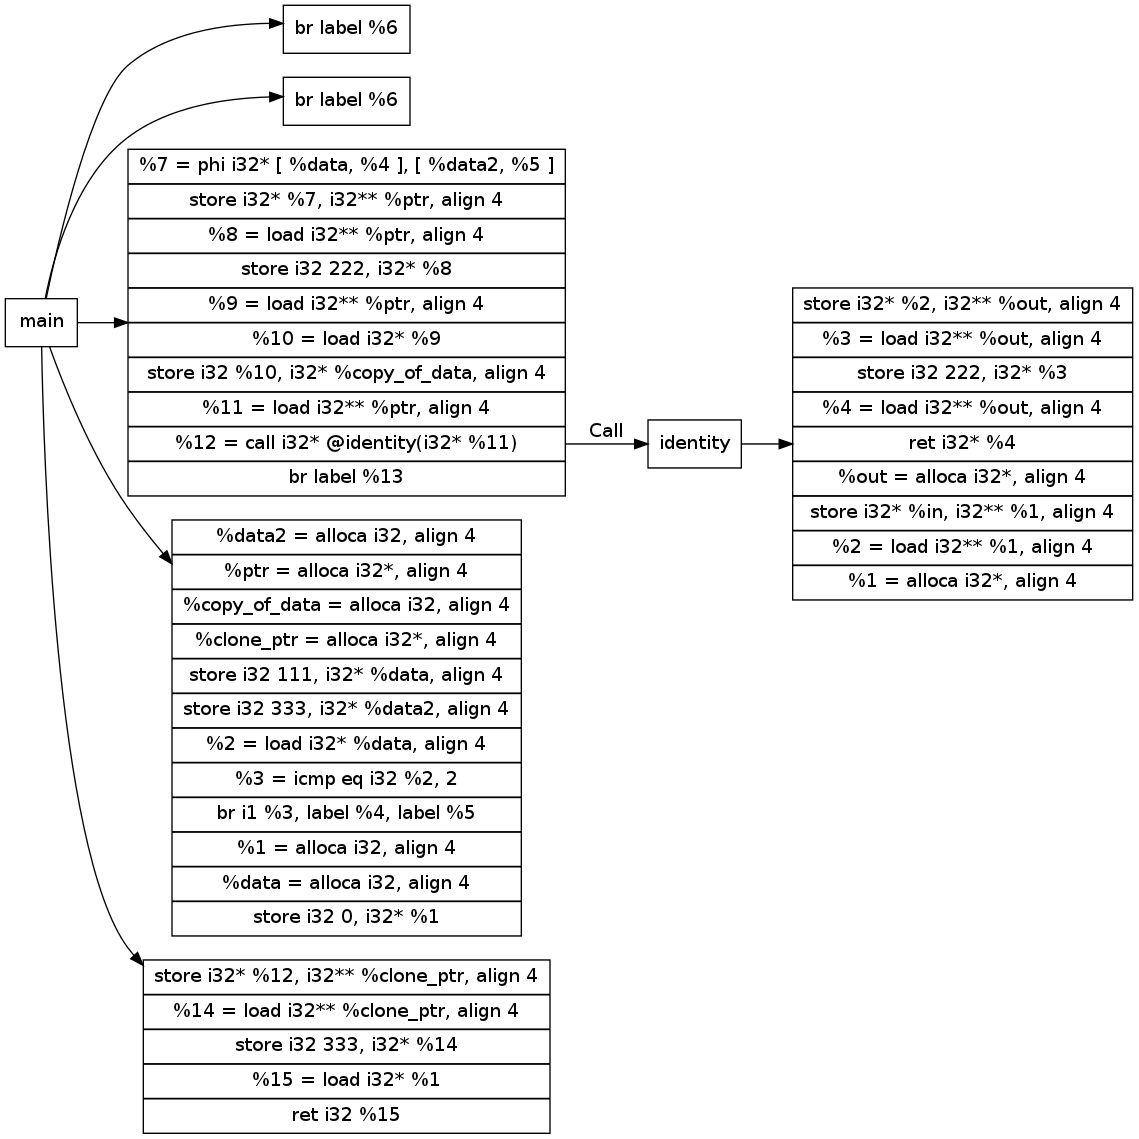
\includegraphics[scale=0.4]{images/passes4.png}
\end{center}
\caption{Example Visualization of a Code Block}
\label{fig:passes4-vis}
\end{figure}



%%%%%%%%%%%%%%%%%%%%%%%%%%%%%%%%%%%%%%%%%%%%%%%%%%%%%%%%%%%%%%%%%%%%%%%%%%%%%%%%

\section{Results}

\subsection{Flow-Sensitivity and Flow-Insensitivity}
To show that our flow-insensitive and flow sensitive analyses work, consider the following code
snippet in Figure \ref{fig:fi-code}.

\begin{figure}
\begin{center}
\leavevmode
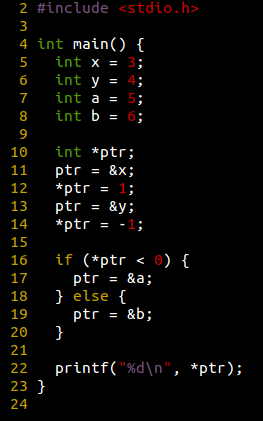
\includegraphics[scale=0.5]{images/fi_example_code.png}
\end{center}
\caption{Flow-Insensitive Code Example}
\label{fig:fi-code}
\end{figure}

A flow-sensitive analysis should produce that, at the end of the program,
\code{ptr} points only to \code{a} and \code{b}. However, a flow-insensitive
manuever would show that \code{ptr} could point to any of \code{a}, \code{b},
\code{c}, and \code{d}. (Note that we do not use the thesis's version of flow-
insensitivity here; we do a regular flow-insensitive solution). In Figures
\ref{fig:fi-log} and \ref{fig:fs-log} we see that this is exactly what has
happened.

\begin{figure}
\begin{center}
\leavevmode
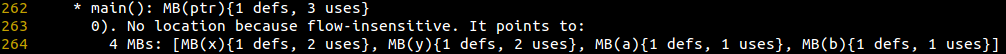
\includegraphics[scale=0.5]{images/fi_log.png}
\end{center}
\caption{Flow-Insensitive Solution}
\label{fig:fi-log}
\end{figure}

\begin{figure}
\begin{center}
\leavevmode
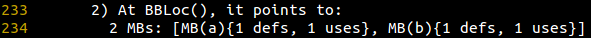
\includegraphics[scale=0.5]{images/fs_log.png}
\end{center}
\caption{Flow-Sensitive Solution}
\label{fig:fs-log}
\end{figure}

\subsection{Context-Sensitivity and Context Insensitivity}
To show that our context-insensitive and context sensitive solutions functions
properly, consider the code snippet in Figure \ref{fig:ci-code}.

\begin{figure}
\begin{center}
\leavevmode
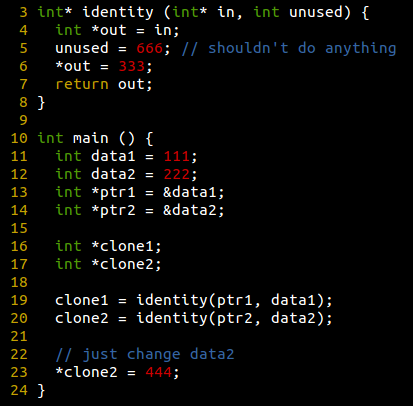
\includegraphics[scale=0.5]{images/ci_code.png}
\end{center}
\caption{Context-Insensitive Code Example}
\label{fig:ci-code}
\end{figure}

A context-insensitive solution will smear together arguments from calling
functions, and also smear return values. It keeps track of only instance of the
procedure and does not clone on every call. A context-sensitive solution,
however, would clone the procedures on every call and keep a more complicated
representation. The consequences of this are shown in Figures \ref{fig:smear-ci}
and \ref{fig:smear-cs}. The assignment at the end to the pointer \code{clone2}
in Figure \ref{fig:ci-code} combined with a context-insensitive solution would
dictate that now either \code{ptr1} or \code{ptr2} can be $444$. A
context-sensitive solution, however, would not lose precision here.

\begin{figure}
\begin{center}
\leavevmode
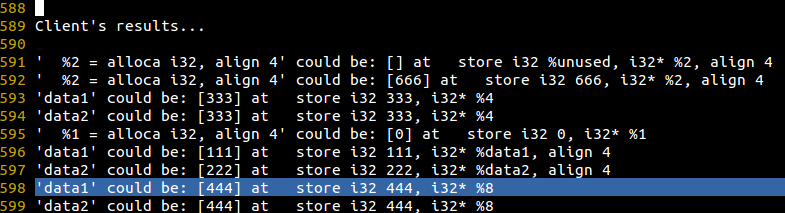
\includegraphics[scale=0.5]{images/smear_ci.png}
\end{center}
\caption{Context-Insensitive Smearing Arguments}
\label{fig:smear-ci}
\end{figure}

\begin{figure}
\begin{center}
\leavevmode
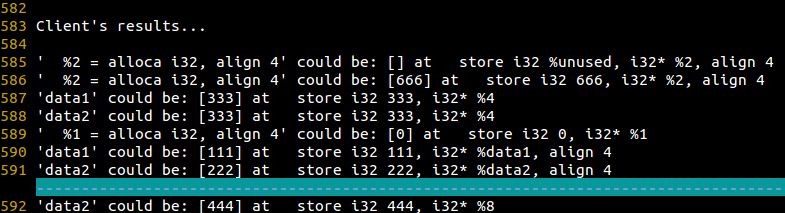
\includegraphics[scale=0.5]{images/smear_cs.png}
\end{center}
\caption{Context-Sensitive Smearing Arguments}
\label{fig:smear-cs}
\end{figure}


In addition to that, a look into the bowels of our debugging output in Figures
\ref{fig:calling-ci} and \ref{fig:calling-cs} will show that when looking for a
def of \code{data2}, the location trees are significantly different for the
context-sensitive and context-insensitive version. In particular, the
context-insensitive version does not have a ``called by'' portion like the
context-sensitive version does.

\begin{figure}
\begin{center}
\leavevmode
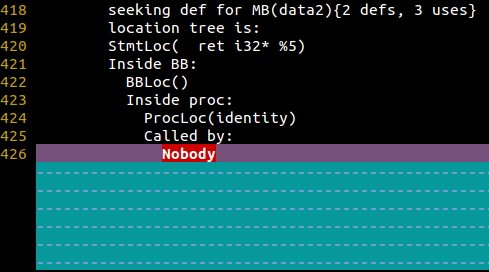
\includegraphics[scale=0.5]{images/calling_ci.png}
\end{center}
\caption{Context-Insensitive Location Tree}
\label{fig:calling-ci}
\end{figure}

\begin{figure}
\begin{center}
\leavevmode
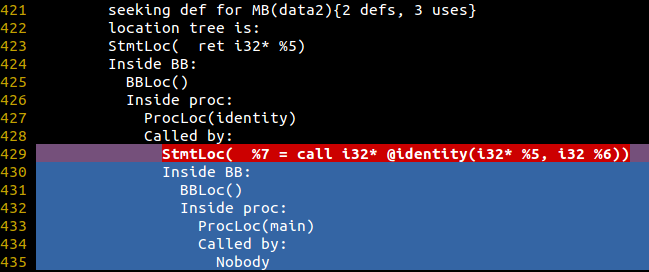
\includegraphics[scale=0.5]{images/calling_cs.png}
\end{center}
\caption{Context-Sensitive Location Tree}
\label{fig:calling-cs}
\end{figure}

%%%%%%%%%%%%%%%%%%%%%%%%%%%%%%%%%%%%%%%%%%%%%%%%%%%%%%%%%%%%%%%%%%%%%%%%%%%%%%%%

\section{Limitations}

Due to time constraints, there are some limitations with the parts of the
analysis that we did implement:

\begin{itemize}
\item Client analyses should be able to specify forwards or backwards analysis,
      but we are currently fixed at forwards.
\item We have not tested our analysis on IR generated from anything other than
      ``clang -O0''. Theoretically any valid IR should work, but mapping C-level
      operations to LLVM IR is sometimes tricky. We had particular difficulties
      distinguishing pointer dereferences from pointer copies.
\item On that note, we have only ever tested and reasoned about C. C++ and other
      source languages may work if the IR generated is similar.
\item Guyer's thesis mentions ``multiple instance analysis'', an IDFA performed
      to determine if a malloc must represent exactly one memory block at runtime.
      This permits strong updates on some heap blocks. We did not attempt this.
\item Procedures must be analyzed conservatively in the presence of indirect
      function pointers and recursion. We detect these cases and do no analysis. This
      was not tested.
\item Context- and flow-insensitive modes were not tested as heavily as the
      sensitive modes. In particular, we do not have any tests involving loops.
\end{itemize}

%%%%%%%%%%%%%%%%%%%%%%%%%%%%%%%%%%%%%%%%%%%%%%%%%%%%%%%%%%%%%%%%%%%%%%%%%%%%%%%%

\section{Future Work}

We did not reach several major goals:

\begin{itemize}
\item integrate with client DFA by associating flow values with defs, as well as
      points-to sets
\item creating defs and uses that annotations specify when we call a library
      function
\item the Monitor and Adaptor. It was difficult to trace sources of imprecision
      before integrating with the client analysis.
\end{itemize}

Aside from these original goals, we have broader visions for extensions.

\subsection{Refactoring}

With many collaborators and a rapid development schedule, the code has outgrown
our initial design sketches. There have been, to say it colloquially, hacks upon
hacks that we have implemented to interface our code with one anothers. For
instance there are globals littered in different files, and a need for a more
sustainable debugging system. Problems as simple as differing naming conventions
make portions of the code difficult to read.

More generally, the problem is that there are no unifying design principles
guiding our code. We believe this is a priority before we move too much further,
to ensure that our code does not become an unmaintainable mess.

In addition to simple refactoring, there are places where we are not fully using
to our advantage the power of LLVM. We believed it would be simpler to work on
our own code, but there already exists an \code{AliasAnalysis} interface in LLVM
that we may have used \cite{aliasanalysis} . Our knowledge of LLVM going into
the project was very minimal, so using what we've learned we can harness more
tools that LLVM offers. The \code{AliasAnalysis} interface may be wise to
eventually implement if we open-source this work, so other clients can use our
pointer analysis.

Now that we have a more sophisticated understanding of the architecture of the
system, there are certainly changes we could make to improve clarity. One
example where we chose to do this anyway was the list of phi merge functions per
memory block. Guyer's thesis stores these per block, but the reference implementation
moves these to the Procedure DB.  This creates a chain of calls that is much
harder to follow, so after we determined this structuring does not cause any
different semantics, we chose the straightforward choice of storing phis in each
block in our implementation.

\subsection{Testing (at scale)}

In the time that we had, we were unable to incorporate larger and more
substantial tests. More than that, there is a need to ensure that the
fundamental components work as expected. One improvement we plan to make in the
future is to add in a more comprehensive testing suite, one that will allow us
to verify correctness more simply. This will also allow us to then make changes
and then verify that our changes worked with confidence. This is a high
priority, and will be imperative as we move forward in this project. 

We also had thoughts about automatically generating example C with randomized
interleavings of procedure calls, branches, and levels of pointer dereference.
In a higher level language operating at a much higher level of abstraction
(since the code output is a function of the program data we generate),
performing the same pointer manuever might be much easier to verify. This means
we could compare the results between the two implementations automatically.

\subsection{Open Source}

It is our vision that one day others can benefit and improve upon the ideas that
Broadway put forth. We plan to open source the project once it is in a good
enough state, and let the community contribute changes. We developed a pass to
split Basic Blocks at procedure calls so that placing virtual phi functions can
be done more consistently. We also ported a pass to compute the ancestors of a
function (all callers of it, flattened from the usual call graph). Both would be
generally reusable.

\subsection{Optimization}

The LLVM Programmer's Manual recommends different implementations of sets and
maps based on precisely what they store \cite{llvmprogdoc}. We chose to use STL
data structures because they work immediately, while the LLVM specializations
have poor documentation, no simple examples, and have a higher initial learning
curve. A simple improvement is to use specialized structures instead.

\subsection{Staged Analysis}

There has been related work to perform F.S. pointer analysis much more quickly
by performing a conservative, fast auxiliary analysis before the main pass
\cite{cc06}.  Although Broadway does something similar, it still adds all
reachable basic blocks to the worklist upon changes. It should be possible to
merge these two ideas and create a much less redundant main pass that re-visits
less blocks.

%%%%%%%%%%%%%%%%%%%%%%%%%%%%%%%%%%%%%%%%%%%%%%%%%%%%%%%%%%%%%%%%%%%%%%%%%%%%%%%%

\section{Appendix A: Build instructions}
The entirety of the source code can be found at the following link:
\url{https://bitbucket.org/aluong/broadway/}. Please let us know if you cannot
get access to the repository.

\subsection{Dependences}
We assume the following about your system.

\begin{itemize}
\item You have compiled your own version of LLVM (living in
  \code{LLVM-ROOT-DIR})
\item You are working in a *nix environment
\item \code{clang} is installed
\item \code{mercurial} (\code{hg}) is installed
\end{itemize}

Wherever your system may deviate from this, adjust our instructions accordingly.

\subsection{Obtaining the Source}

To get our source code, ensure that you have mercurial installed on your system
and run: 
$$\text{\code{hg clone https://bitbucket.org/aluong/broadway}}$$
For simplicity, we would recommend you run this clone command from\\
\code{LLVM-ROOT-DIR/lib/Analysis}.

\subsection{Compiling}

Once you have the code, open up \code{build.sh}. Edit the shell variable
\code{\$LLVM\_RELEASE\_TYPE} to match your release type. Then \code{chmod +x
build.sh} if necessary, and run the script. It may spit out an absurd
number of warnings, but that is okay. They are not from our code.

\subsection{Running}

We have a couple scripts present that we used when developing, that you can use
to test/run the code.  The script \code{testlogs.sh} will run all the c programs
in the \code{tests/} directory and produce output for all of them into the
\code{logs/} direcotry. The script \code{test\_fi.sh} will run all the
\code{passes*.c} tests in the \code{tests/} folder, and produce output in the
logs; one file for a flow-insensitive run, and one file for a flow-insensitve
run. And lastly, there is a \code{combinecommand} script that runs a taintedness
test on \code{AnnotationPass/test/taintedness-test1.c}. There is also a
\code{test\_fi.sh}, but it has been failing some recent tests.
If running opt manually, note that the \code{-split-at-call} pass must be run before the
\code{-main} pass for our assumptions to hold. \code{addRequired<SplitPass>} did not seem
to do what we wanted in that respect, but it does work this way. 


%%%%%%%%%%%%%%%%%%%%%%%%%%%%%%%%%%%%%%%%%%%%%%%%%%%%%%%%%%%%%%%%%%%%%%%%%%%%%%%%
\newpage
\bibliographystyle{plain}
\bibliography{sources}

\end{document}
